\section{Introduction to Fault Attacks}
\begin{frame}{\VideoName}
    \tableofcontents[currentsection]
\end{frame}

\begin{frame}{High Level Description of Fault Attacks}
    \begin{itemize}
        \item Active attacks, the attacker tries to perturb the internal computations by external means
        \item Exploit a scenario where the attacker has access to the device and can tamper with it
        \item There exist also techniques that can achieve fault attacks remotely, such as Rowhammer\footnote{Kim, Yoongu, et al. "Flipping bits in memory without accessing them: An experimental study of DRAM disturbance errors." ACM SIGARCH Computer Architecture News 42.3 (2014): 361-372.}
    \end{itemize}
    
    \begin{tikzpicture}[remember picture,overlay]
    \node[xshift=-2cm,yshift=2.3cm] at (current page.south east) {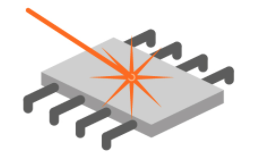
\includegraphics[width = 0.3\textwidth]{fig/FaultAttacksFigure.png}};
    \node[xshift=-3cm,yshift=0.2cm] at (current page.south east)
    {\tiny{picture source: \url{https://blog.applus.com/}}};
    \end{tikzpicture}
\end{frame}

\begin{frame}{Fault Injection Techniques}
\begin{figure}
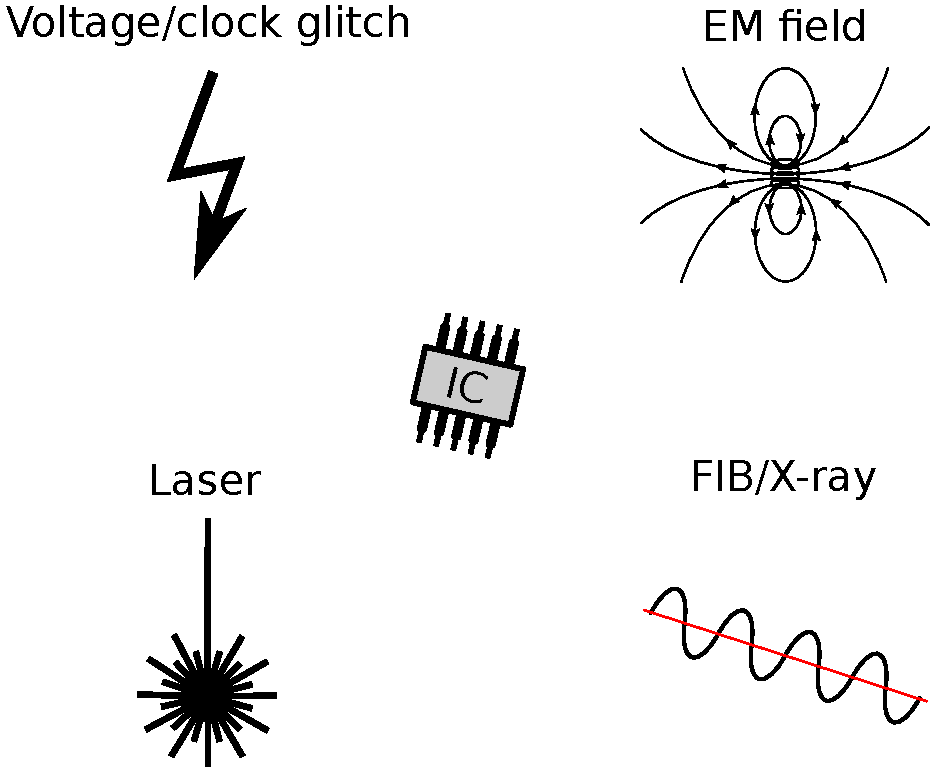
\includegraphics[width=0.7\textwidth]{fig/FA_techniques}
\end{figure}
\end{frame}

% \begin{frame}{Laser Fault Injection Setup}
% %%Columns-----
% \begin{columns}
% \begin{column}{.5\textwidth}
% By carefully tuning the beam’s energy level below a destructive threshold, it is possible to inject faults into a device and it will not suffer any permanent damage
% \end{column}%
% \hfill%
% \begin{column}{.5\textwidth}
% \begin{figure}[h!] \centering
% 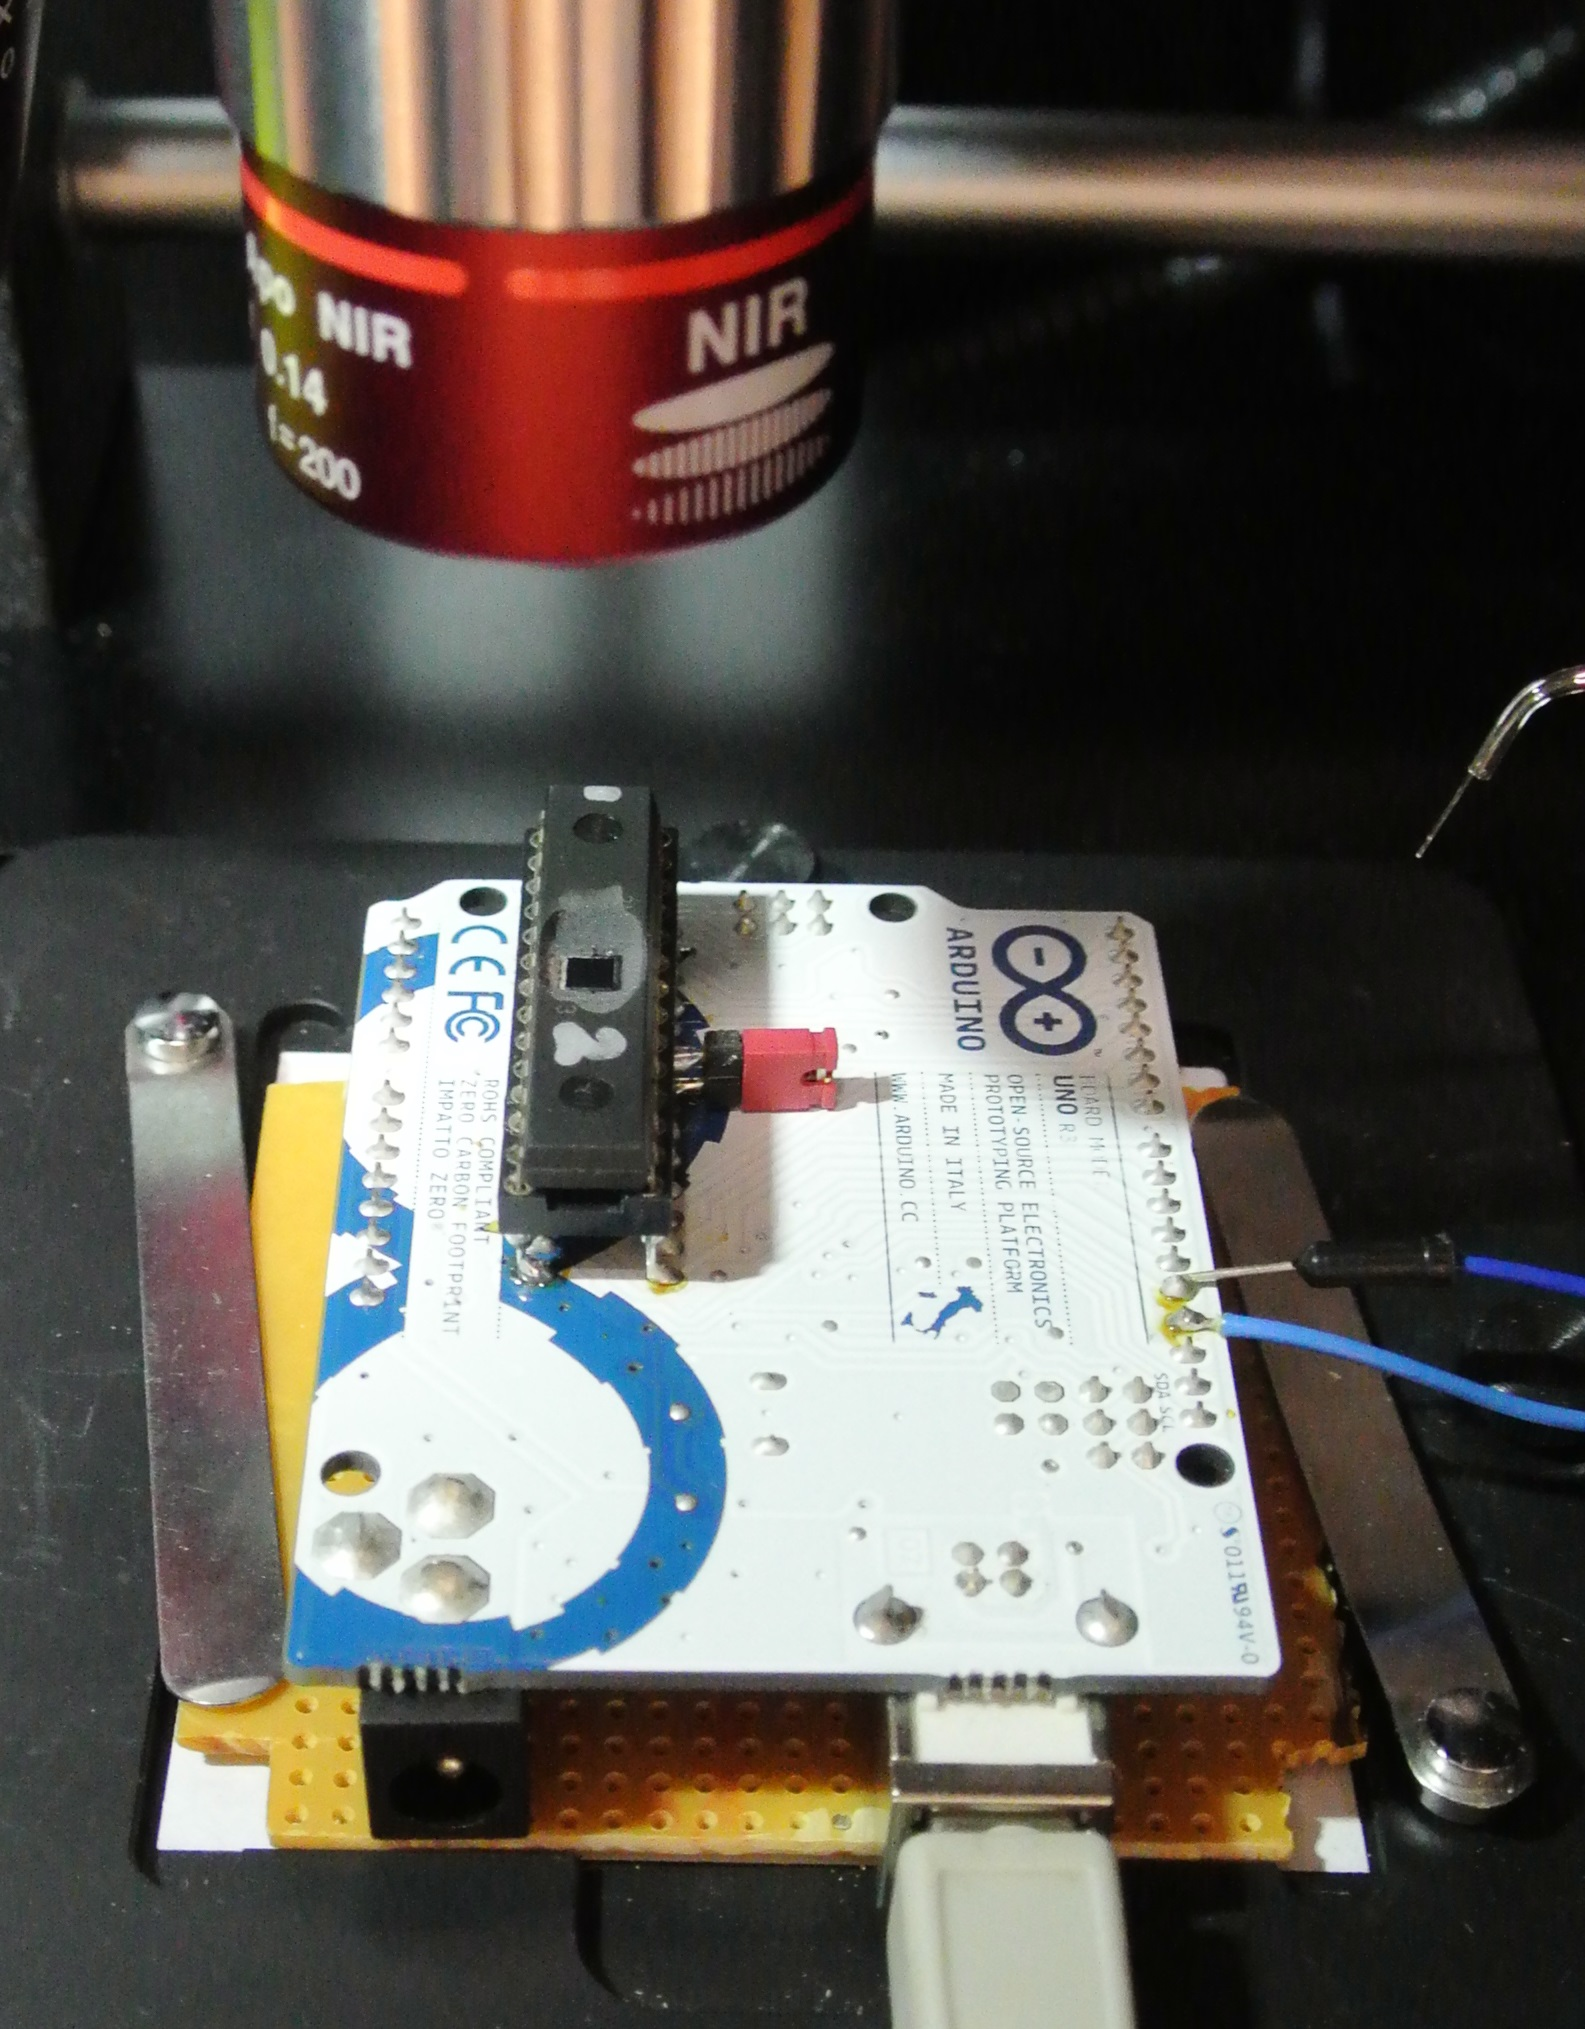
\includegraphics[width=0.8\textwidth]{fig/laser_setup}
% \end{figure}
% \end{column}%
% \end{columns}
% \end{frame}

\begin{frame}{Fault Effects}
    \begin{itemize}
        \item Instruction skip/change
        \begin{itemize}
            \item perturbs the instruction being executed by modifying the opcode for the instruction
        \end{itemize}
        \item Bit flip
        \begin{itemize}
            \item Flips the bits in the data.
             \item The number of bits affected is normally limited by the size of the registers.
             \item For example, for an 8-bit device, we can have $m-$bit flips for $m=1,2,\dots,8$
        \end{itemize}
        \item Bit set/reset
        \begin{itemize}
            \item fixes the bit value to be $1$ (set) or $0$ (reset)
        \end{itemize}
        \item Random byte fault
        \begin{itemize}
            \item changes the byte value to a random number
        \end{itemize}
        \item Stuck-at faults
        \begin{itemize}
            \item permanently changes the value of one bit to $0$ (stuck-at-$0$) or $1$ (stuck-at-$1$)
        \end{itemize}
        \item ...
    \end{itemize}
\end{frame}

\begin{frame}{Fault Types}
    \begin{itemize}
        \item \textit{permanent fault} 
        \begin{itemize}
            \item destructive fault that changes the value of a memory cell permanently and hence affects data during the computations
        \end{itemize}
        \item \textit{transient fault}
        \begin{itemize}
            \item the circuit recovers its original behavior after the fault stimulus ceases (usually just one instruction) or after the device reset
            \item can perturb both data and instruction
        \end{itemize}
        \item In this course, we only consider transient faults
    \end{itemize}
\end{frame}

\begin{frame}{First Fault Attack}
    \begin{itemize}
         \item Introduced by Boneh et al. to attack implementation of RSA with CRT\footnote{Boneh, D., DeMillo, R. A., \& Lipton, R. J. (1997, May). On the importance of checking cryptographic protocols for faults. In International conference on the theory and applications of cryptographic techniques (pp. 37-51). Springer, Berlin, Heidelberg.}
        \item After the fault injection, there are two possible scenarios
        \begin{itemize}
            \item the output (ciphertext) is faulty
            \item fault is ineffective and the ciphertext is not changed
            \item both scenarios can be exploited
        \end{itemize}
        \item Attacker goal: recover private key
        \item Developed on the algorithmic level
        \item There are also implementation-specific vulnerabilities
    \end{itemize}
\end{frame}

\begin{frame}{Fault attacks on symmetric block ciphers}
    \begin{itemize}
        \item The specifications of round functions and key schedules are public (Kerckhoffs' principle)
       \item The master key, hence also the round keys, are secret.
        \item We also assume that throughout the attack, the same master key is used and the goal of the attacker is normally to recover certain round key(s).
         \item The methodologies that we will discuss can be applied to any unprotected implementations of symmetric block cipher proposed up to now
         \item Fault attacks normally aim to recover the last/first round key(s), then use the inverse key schedule to find the master key
        \begin{itemize}
            \item DES: any round key $\to$ $48$ bits of master key
            \item AES: any round key $\to$ master key
            \item PRESENT: any round key $\to$ $64$ bits of master key, brute force the rest or recover another round key
        \end{itemize}
    \end{itemize}
\end{frame}

\begin{frame}{Fault mask}
    \begin{itemize}
        \item If the fault injected in an intermediate value $x$, it changes to a faulty value $x'$
        \item We refer to $\varepsilon:=x\oplus x'$ as the \textit{fault mask}, which represents the change in the faulted value.
    \end{itemize}
\end{frame}

\section{Differential Fault Analysis}
\begin{frame}{\VideoName}
    \tableofcontents[currentsection]
\end{frame}

\begin{frame}{Attack methodology}
    \begin{itemize}
        \item Differential Fault Analysis (DFA) was first introduced by Biham et al.~\footnote{Biham, E., \& Shamir, A. (1997, August). Differential fault analysis of secret key cryptosystems. In Annual international cryptology conference (pp. 513-525). Springer, Berlin, Heidelberg.} in 1997.
       \item It has been studied by numerous researchers in different settings and is one of the most popular fault attack analysis methods for symmetric block ciphers.
       \item DFA considers a fault injection into the intermediate state of the cipher, normally in the last few rounds.
       \item Then the difference between correct and faulty ciphertexts is analyzed to recover the round key(s).
    \end{itemize}
\begin{figure}
    \centering
    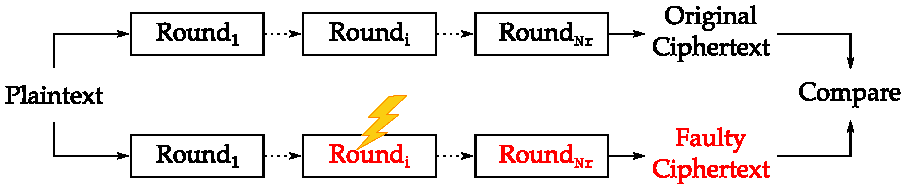
\includegraphics[width=0.8\textwidth]{fig/dfa}
    % \caption{Caption}
\end{figure}
\end{frame}

\begin{frame}{Difference distribution table}
    \begin{definition}
    For an Sbox SB$:\FF_2^{\omega_1}\to\FF_2^{\omega_2}$, the \textit{(extended) difference distribution table (DDT)} of SB is a $2-$dimensional table $T$ of size $(2^{\omega_1}-1)\times2^{\omega_2}$ such that for any $0<\delta<2^{\omega_1}$ and $0\leq\Delta<2^{\omega_2}$, the entry of $T$ at the $\Delta$th row and $\delta$th column is given by
    \[
    T[\Delta,\delta]=\Set{\boldsymbol{a}\ |\ \boldsymbol{a}\in\FF_2^{\omega_1}, \text{SB}(\boldsymbol{a}\oplus \delta)\oplus \text{SB}(\boldsymbol{a)}=\Delta}.
    \]
    We refer to $\delta$ as the \textit{input difference}, and $\Delta$ as the \textit{output difference}.
\end{definition}
\begin{example}[DDT of PRESENT Sbox]
\begin{table}
\begin{tabular}{cccccccccccccccc}\hline
0 & 1 & 2 & 3 & 4 & 5 & 6 & 7 & 8 & 9 & A & B & C & D & E & F \\
C & 5 & 6 & B & 9 & 0 & A & D & 3 & E & F & 8 & 4 & 7 & 1 & 2\\\hline
\end{tabular}
\end{table}
If input is \texttt{9}, input difference $\delta=\texttt{3}$, the output difference is given by
\[
\text{SB}_{\text{PRESENT}}(\texttt{9}\oplus \texttt{3})\oplus \text{SB}_{\text{PRESENT}}(\texttt{9})=\text{SB}_{\text{PRESENT}}(\texttt{A})\oplus1110=1111\oplus1110=0001=\texttt{1}.
\]
\end{example}
\end{frame}

\begin{frame}{Difference distribution table}
    \begin{definition}
    For an Sbox SB$:\FF_2^{\omega_1}\to\FF_2^{\omega_2}$, the \textit{(extended) difference distribution table (DDT)} of SB is a $2-$dimensional table $T$ of size $(2^{\omega_1}-1)\times2^{\omega_2}$ such that for any $0<\delta<2^{\omega_1}$ and $0\leq\Delta<2^{\omega_2}$, the entry of $T$ at the $\Delta$th row and $\delta$th column is given by
    \[
    T[\Delta,\delta]=\Set{\boldsymbol{a}\ |\ \boldsymbol{a}\in\FF_2^{\omega_1}, \text{SB}(\boldsymbol{a}\oplus \delta)\oplus \text{SB}(\boldsymbol{a)}=\Delta}.
    \]
    We refer to $\delta$ as the \textit{input difference}, and $\Delta$ as the \textit{output difference}.
\end{definition}
\begin{example}[DDT of PRESENT Sbox]
\begin{table}
\begin{tabular}{cccccccccccccccc}\hline
0 & 1 & 2 & 3 & 4 & 5 & 6 & 7 & 8 & 9 & A & B & C & D & E & F \\
C & 5 & 6 & B & 9 & 0 & A & D & 3 & E & F & 8 & 4 & 7 & 1 & 2\\\hline
\end{tabular}
\end{table}
If input is \texttt{9}, input difference $\delta=\texttt{3}$, the output difference is given by \texttt{1}.
Thus \texttt{9} is in $T[\texttt{1},\texttt{3}]$.
\end{example}
\end{frame}

\begin{frame}{DDT of PRESENT Sbox}
\begin{table} 
\centering
\ttfamily
\resizebox{1.0\textwidth}{!}{
\begin{tabular}{|c|ccccccccccccccc|}\hline
\backslashbox{$\Delta$}{$\delta$} & 1 & 2 & 3 & 4 & 5 & 6 & 7 & 8 & 9 & A & B & C & D & E & F \\ \hline\hline
1 &   &   & 9A &   & 36 &   & 078F &   &   &   & 5E &   & 1C &   & 24BD \\ \hline
2 &   &   &   &   &   & 8E & 34 &   & 09 & 5F &   & 1D & 67AB & 2C &   \\ \hline
3 & CDEF & 46 & 12 &   &   &   &   & 3B &   & 0A &   &   & 58 & 79 &   \\ \hline
4 &   &   & 47 &   & 8D &   &   &   & 35AC &   & 0B &   & 2F &   & 169E \\ \hline
5 &   & CDEF &   & 0145 &   &   &   &   &   & 2389 &   & 67AB &   &   &   \\ \hline
6 &   & 9B & CDEF & 37 &   & 06 & 25 &   & 18 &   &   &   &   & 4A &   \\ \hline
7 & 67AB &   & 03 & 8C &   &   &   & 5D &   &   &   & 2E & 49 & 1F &   \\ \hline
8 &   &   &   &   &   & 17 & AD &   & 6F & 4E & 2389 & 0C &   & 5B &   \\ \hline
9 & 0145 &   &   & 9D & BE &   &   & 2A &   &   & 7C & 3F &   & 68 &   \\ \hline
A &   & 02 & 56 & BF & 9C &   &   &   &   & 7D & 1A & 48 & 3E &   &   \\ \hline
B &   &   & 8B &   & 27 & 35AC &   & 169E &   &   & 4F &   & 0D &   &   \\ \hline
C &   & 8a &   & 26 & 0145 & 9F & BC &   & 7E &   &   &   &   & 3D &   \\ \hline
D & 2389 & 57 &   &   & AF &   &   & 4C &   & 1B & 6D &   &   & 0E &   \\ \hline
E &   & 13 &   & AE &   &   &   &   & 24BD & 6C &   & 59 &   &   & 078F \\ \hline
F &   &   &   &   &   & 24BD & 169E & 078F &   &   &   &   &   &   & 35AC \\ \hline
\end{tabular}
}
\caption{Difference distribution table for PRESENT Sbox, where the row corresponding to output difference $\Delta=\texttt{0}$ is omitted since it is empty}
\end{table}
\end{frame}

\begin{frame}{How DFA works on a simple example}
\begin{itemize}
    \item  Let us consider the \texttt{AND} operation that takes inputs $a, b\in\FF_2$ and outputs
    \[
    c=a\ \& \ b.
    \]
    \item  All possible values of $a,b,c$ are given by
    \begin{center}
        \begin{tabular}{|c|c|c|}\hline
$a$ & $b$ & $c = a \ \&\ b$ \\ \hline
0 & 0 & 0  \\
0 & 1 & 0  \\ \hline
1 & 0 & 0  \\
1 & 1 & 1  \\ \hline
\end{tabular}
    \end{center}
\item Suppose the output $c$ can be observed by the attacker and $a,b$ are unknown.
\item The attacker injects a fault in $b$ by flipping it.
\item If the output $c$ stays the same, then $a=0$; otherwise $a=1$.
\end{itemize}
\end{frame}

\begin{frame}{How DFA works on PRESENT Sbox}
    \begin{itemize}
       \item SB: PRESENT Sbox
        \item Let $\boldsymbol{a}\in\FF_2^4,\ \boldsymbol{b}\in\FF_2^4$ be fixed secret values
        \item Define
\begin{eqnarray*}
    f:\FF_2^4&\to&\FF_2^4\\
    \boldsymbol{x}&\mapsto& \text{SB}(\boldsymbol{x}\oplus\boldsymbol{a})\oplus\boldsymbol{b}.\nonumber
\end{eqnarray*}
\item We will show how to recover the values of $\boldsymbol{a}$ and $\boldsymbol{b}$ with DFA
\item Attack assumption
\begin{itemize}
     \item Fault location: input of $f$
    \item Fault model: bit flip
    \item Fault mask: $\varepsilon\in\FF_2^4$ s.t. $\boldsymbol{x}'=\boldsymbol{x}\oplus\varepsilon$
        \item Attacker knowledge: Sbox design, inputs and outputs of $f$, fault mask
        \item Attacker goal: recover values of $\boldsymbol{a}$ and $\boldsymbol{b}$
        \item Attacker can repeat the computation with the same input (not chosen by attacker)
\end{itemize}
    \end{itemize}
\end{frame}

\begin{frame}{How DFA works on PRESENT Sbox}
\begin{eqnarray*}
    f:\FF_2^4&\to&\FF_2^4\\
    \boldsymbol{x}&\mapsto& \text{SB}(\boldsymbol{x}\oplus\boldsymbol{a})\oplus\boldsymbol{b}.
\end{eqnarray*}
    \begin{itemize}
\item Attack assumption
\begin{itemize}
     \item Fault location: input of $f$
    \item Fault model: bit flip
    \item Fault mask: $\varepsilon\in\FF_2^4$ s.t. $\boldsymbol{x}'=\boldsymbol{x}\oplus\varepsilon$
        \item Attacker knowledge: Sbox design, inputs and outputs of $f$, fault mask
        \item Attacker goal: recover values of $\boldsymbol{a}$ and $\boldsymbol{b}$
        \item Attacker can repeat the computation with the same input (not chosen by attacker)
\end{itemize}
\item Attack steps:
\begin{itemize}
    \item Compute DDT of the Sbox, $T$
    \item Inject fault
    \item Reduce guesses for $\boldsymbol{a}$ with knowledge of fault mask, input and outputs
    \item Reduce guesses for $\boldsymbol{b}$ with guesses of $\boldsymbol{a}$, knowledge of the correct input and output
\end{itemize}
    \end{itemize}
\end{frame}

\begin{frame}{How DFA works on PRESENT Sbox}
\begin{eqnarray*}
    f:\FF_2^4&\to&\FF_2^4\\
    \boldsymbol{x}&\mapsto& \text{SB}(\boldsymbol{x}\oplus\boldsymbol{a})\oplus\boldsymbol{b}.\nonumber
\end{eqnarray*}
 Attack steps:
\begin{itemize}
    \item Compute DDT of the Sbox, $T$
    \item Inject fault
    \item Reduce guesses for $\boldsymbol{a}$ with knowledge of fault mask, input and outputs
    \begin{itemize}
         \item Let $\Delta$ denote the difference between the correct and faulty output, then
\begin{equation*}
    \Delta=(\text{SB}(\boldsymbol{x}\oplus\boldsymbol{a})\oplus\boldsymbol{b})\oplus(\text{SB}(\boldsymbol{x}'\oplus\boldsymbol{a})\oplus\boldsymbol{b})
    =\text{SB}(\boldsymbol{x}\oplus\boldsymbol{a})\oplus\text{SB}(\boldsymbol{x}'\oplus\boldsymbol{a})=\text{SB}(\boldsymbol{x}\oplus\boldsymbol{a})\oplus\text{SB}(\boldsymbol{x}\oplus\boldsymbol{a}\oplus\varepsilon)
\end{equation*} 
\item Thus the value $\boldsymbol{x}\oplus\boldsymbol{a}$ is in the entry of $T$ corresponding to input difference $\delta=\varepsilon$ and output difference $\Delta$
    \end{itemize}
    \item Reduce guesses for $\boldsymbol{b}$ with guesses of $\boldsymbol{a}$, knowledge of the correct input and output
\end{itemize}
\end{frame}

\begin{frame}{How DFA works on PRESENT Sbox -- Example}
\begin{eqnarray*}
    f:\FF_2^4&\to&\FF_2^4\\
    \boldsymbol{x}&\mapsto& \text{SB}(\boldsymbol{x}\oplus\boldsymbol{a})\oplus\boldsymbol{b}.\nonumber
\end{eqnarray*}
Reduce guesses for $\boldsymbol{a}$ with knowledge of fault mask, input and outputs
    \begin{itemize}
         \item Let $\Delta$ denote the difference between the correct and faulty output, then
{\small
\begin{equation*}
    \Delta=(\text{SB}(\boldsymbol{x}\oplus\boldsymbol{a})\oplus\boldsymbol{b})\oplus(\text{SB}(\boldsymbol{x}'\oplus\boldsymbol{a})\oplus\boldsymbol{b})
    =\text{SB}(\boldsymbol{x}\oplus\boldsymbol{a})\oplus\text{SB}(\boldsymbol{x}'\oplus\boldsymbol{a})=\text{SB}(\boldsymbol{x}\oplus\boldsymbol{a})\oplus\text{SB}(\boldsymbol{x}\oplus\boldsymbol{a}\oplus\varepsilon)
\end{equation*}}
\item Thus the value $\boldsymbol{x}\oplus\boldsymbol{a}$ is in the entry of $T$ corresponding to input difference $\delta=\varepsilon$ and output difference $\Delta$
    \end{itemize}
    \begin{example}
        \begin{itemize}
           \item Suppose the attacker fixes the input to be $\boldsymbol{x}=\texttt{0}$ and they know that the correct output of $f$ is \texttt{0}
            \item When the attacker injects fault in $\boldsymbol{x}$ with fault mask $\varepsilon_1=\texttt{3}$, they get a faulty output \texttt{1}, which gives             
            $\Delta_1=\texttt{0}\oplus\texttt{1}=\texttt{1}$.
            % \item $\boldsymbol{x}\oplus\boldsymbol{a}=\boldsymbol{a}$ is in the entry corresponding to input difference $\delta=?$ and output difference ? of $T$
        \end{itemize}
    \end{example}
\end{frame}

\begin{frame}{How DFA works on PRESENT Sbox -- Example}
\begin{table} 
\centering
\ttfamily
\resizebox{1.0\textwidth}{!}{
\begin{tabular}{|c|ccccccccccccccc|}\hline
\backslashbox{$\Delta$}{$\delta$} & 1 & 2 & 3 & 4 & 5 & 6 & 7 & 8 & 9 & A & B & C & D & E & F \\ \hline\hline
1 &   &   & 9A &   & 36 &   & 078F &   &   &   & 5E &   & 1C &   & 24BD \\ \hline
2 &   &   &   &   &   & 8E & 34 &   & 09 & 5f &   & 1D & 67AB & 2C &   \\ \hline
3 & CDEF & 46 & 12 &   &   &   &   & 3B &   & 0A &   &   & 58 & 79 &   \\ \hline
4 &   &   & 47 &   & 8D &   &   &   & 35AC &   & 0B &   & 2F &   & 169E \\ \hline
5 &   & CDEF &   & 0145 &   &   &   &   &   & 2389 &   & 67AB &   &   &   \\ \hline
6 &   & 9B & CDEF & 37 &   & 06 & 25 &   & 18 &   &   &   &   & 4A &   \\ \hline
7 & 67AB &   & 03 & 8C &   &   &   & 5D &   &   &   & 2E & 49 & 1F &   \\ \hline
$\dots$ & $\dots$ & $\dots$ & $\dots$ & $\dots$ & $\dots$ & $\dots$ & $\dots$ & $\dots$ & $\dots$ & $\dots$ & $\dots$ & $\dots$ & $\dots$ & $\dots$ &\\\hline
% 8 &   &   &   &   &   & 17 & AD &   & 6F & 4E & 2389 & 0C &   & 5B &   \\ \hline
% 9 & 0145 &   &   & 9D & BE &   &   & 2A &   &   & 7C & 3F &   & 68 &   \\ \hline
% A &   & 02 & 56 & BF & 9C &   &   &   &   & 7D & 1A & 48 & 3E &   &   \\ \hline
% B &   &   & 8B &   & 27 & 35AC &   & 169E &   &   & 4F &   & 0D &   &   \\ \hline
% C &   & 8a &   & 26 & 0145 & 9f & bc &   & 7e &   &   &   &   & 3d &   \\ \hline
% D & 2389 & 57 &   &   & AF &   &   & 4C &   & 1B & 6D &   &   & 0E &   \\ \hline
% E &   & 13 &   & AE &   &   &   &   & 24BD & 6C &   & 59 &   &   & 078F \\ \hline
% F &   &   &   &   &   & 24BD & 169E & 078F &   &   &   &   &   &   & 35AC \\ \hline
\end{tabular}
}
% \caption{Difference distribution table for PRESENT Sbox, where the row corresponding to output difference $\Delta=\texttt{0}$ is omitted since it is empty}
\end{table}
    \begin{example}
        \begin{itemize}
            \item  Input: $\boldsymbol{x}=\texttt{0}$; correct output: \texttt{0}
            \item fault mask: $\varepsilon_1=\texttt{3}$; faulty output: \texttt{1}, which gives $\Delta_1=\texttt{0}\oplus\texttt{1}=\texttt{1}$.
            \item $\boldsymbol{x}\oplus\boldsymbol{a}$ is in the entry corresponding to input difference $\delta=\texttt{3}$ and output difference \texttt{1} of $T$
            \item The possible values for $\boldsymbol{x}\oplus\boldsymbol{a}$ are \texttt{9} and \texttt{A}
        \end{itemize}
    \end{example}
\end{frame}

\begin{frame}{How DFA works on PRESENT Sbox -- Example}
\begin{eqnarray*}
    f:\FF_2^4&\to&\FF_2^4\\
    \boldsymbol{x}&\mapsto& \text{SB}(\boldsymbol{x}\oplus\boldsymbol{a})\oplus\boldsymbol{b}.\nonumber
\end{eqnarray*}
Reduce guesses for $\boldsymbol{b}$ with guesses of $\boldsymbol{a}$, knowledge of the correct input and output
\begin{table}
\begin{tabular}{cccccccccccccccc}\hline
0 & 1 & 2 & 3 & 4 & 5 & 6 & 7 & 8 & 9 & A & B & C & D & E & F \\
C & 5 & 6 & B & 9 & 0 & A & D & 3 & E & F & 8 & 4 & 7 & 1 & 2\\\hline
\end{tabular}
\end{table}
    \begin{example}
        \begin{itemize}
            \item  Input: $\boldsymbol{x}=\texttt{0}$; correct output: \texttt{0}
            \item fault mask: $\varepsilon_1=\texttt{3}$; faulty output: \texttt{1} $\rightarrow$ the possible values for $\boldsymbol{x}\oplus\boldsymbol{a}$ are \texttt{9} and \texttt{A}
            \item fault mask $\varepsilon_2=\texttt{2}$; faulty output: \texttt{6} $\rightarrow$ possible values for $\boldsymbol{x}\oplus\boldsymbol{a}$ are \texttt{9} and \texttt{B}
            \item $\boldsymbol{a}=\texttt{9}$, $\boldsymbol{b}=\texttt{E}$
        \end{itemize}
    \end{example}
\end{frame}

\begin{frame}{How many faults are needed}
    \begin{table}
\centering
\ttfamily
\resizebox{1.0\textwidth}{!}{
\begin{tabular}{|c|ccccccccccccccc|}\hline
\backslashbox{$\Delta$}{$\varepsilon$} & 1 & 2 & 3 & 4 & 5 & 6 & 7 & 8 & 9 & a & b & c & d & e & f \\ \hline\hline
1 &   &   & 9a &   & 36 &   & 078f &   &   &   & 5e &   & 1c &   & 24bd \\ \hline
2 &   &   &   &   &   & 8e & 34 &   & 09 & 5f &   & 1d & 67ab & 2c &   \\ \hline
3 & cdef & 46 & 12 &   &   &   &   & 3b &   & 0a &   &   & 58 & 79 &   \\ \hline
4 &   &   & 47 &   & 8d &   &   &   & 35ac &   & 0b &   & 2f &   & 169e \\ \hline
5 &   & cdef &   & 0145 &   &   &   &   &   & 2389 &   & 67ab &   &   &   \\ \hline
6 &   & 9b & cdef & 37 &   & 06 & 25 &   & 18 &   &   &   &   & 4a &   \\ \hline
7 & 67ab &   & 03 & 8c &   &   &   & 5d &   &   &   & 2e & 49 & 1f &   \\ \hline
8 &   &   &   &   &   & 17 & ad &   & 6f & 4e & 2389 & 0c &   & 5b &   \\ \hline
9 & 0145 &   &   & 9d & be &   &   & 2a &   &   & 7c & 3f &   & 68 &   \\ \hline
a &   & 02 & 56 & bf & 9c &   &   &   &   & 7d & 1a & 48 & 3e &   &   \\ \hline
b &   &   & 8b &   & 27 & 35ac &   & 169e &   &   & 4f &   & 0d &   &   \\ \hline
c &   & 8a &   & 26 & 0145 & 9f & bc &   & 7e &   &   &   &   & 3d &   \\ \hline
d & 2389 & 57 &   &   & af &   &   & 4c &   & 1b & 6d &   &   & 0e &   \\ \hline
e &   & 13 &   & ae &   &   &   &   & 24bd & 6c &   & 59 &   &   & 078f \\ \hline
f &   &   &   &   &   & 24bd & 169e & 078f &   &   &   &   &   &   & 35ac \\ \hline
\end{tabular}
}
\end{table}
\begin{itemize}
    \item Chosen fault mask: $2$ (e.g. \texttt{3} and \texttt{5})
    \item Random fault mask: at most $4$
\end{itemize}
\end{frame}

\section{Diagonal DFA on AES}
\begin{frame}{\VideoName}
    \tableofcontents[currentsection]
\end{frame}

\begin{frame}{Fault propagation in AES}
    \begin{itemize}
        \item Recall that AES cipher state can be represented as a four-by-four matrix of bytes:
\begin{equation*}
    \begin{pmatrix}
    s_{00} & s_{01} & s_{02} & s_{03}\\
    s_{10} & s_{11} & s_{12} & s_{13}\\
    s_{20} & s_{21} & s_{22} & s_{23}\\
    s_{30} & s_{31} & s_{32} & s_{33}
    \end{pmatrix}.
\end{equation*}
        \item Let us represent those bytes by squares for the purpose of visual illustration.
        \item Suppose a fault is injected at the beginning of one round (except for the last round) in byte $s_{00}$.
        \item Then the fault propagation in this round can be represented by
    \end{itemize}
\begin{figure}
    \centering
    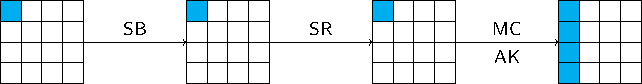
\includegraphics{fig/AES_Fault_Diagnol_Attack_Round8_00.pdf}
    \caption{
    Blue squares correspond to bytes that can be affected by the fault.}
\end{figure}
\end{frame}

\begin{frame}{Fault propagation in AES}
    \begin{figure}
    \centering
    \begin{tabular}{c}
    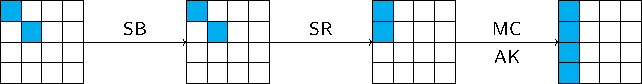
\includegraphics{fig/AES_Fault_Diagnol_Attack_Round8_11.pdf} \\
    (a)\\
    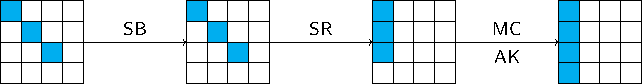
\includegraphics{fig/AES_Fault_Diagnol_Attack_Round8_22.pdf} \\
    (b)\\
    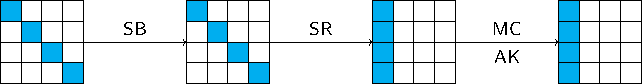
\includegraphics{fig/AES_Fault_Diagnol_Attack_Round8_33.pdf} \\
    (c)
    \end{tabular}
    \caption{Visual illustration of how the fault propagates when a fault is injected at the beginning of one AES round in bytes (a) $s_{00}, s_{11}$, (b) $s_{00}, s_{11}, s_{22}$, and (c) $s_{00}, s_{11}, s_{22}, s_{33}$.
    Blue squares correspond to bytes that can be affected by the fault.}
\end{figure}
\end{frame}

\begin{frame}{Fault at end of round 7}
    \begin{itemize}
        \item Let us refer to the bytes $s_{00}, s_{11}, s_{22}, s_{33}$ as a \textit{diagonal} of AES state
        \item We consider a fault attack where a random byte fault is injected in the diagonal of the AES state at the end of round $7$.
        \item By the above discussion, we know that at the end of round $8$, the whole first column might be affected by the fault.
        \item Similarly, we can study the fault propagation in round $9$.
        \item Recall that MixColumns multiplies one column by the following matrix
\[
\begin{pmatrix}
    \texttt{02} & \texttt{03} & \texttt{01} & \texttt{01} \\
    \texttt{01} & \texttt{02} & \texttt{03} & \texttt{01} \\
    \texttt{01} & \texttt{01} & \texttt{02} & \texttt{03} \\
    \texttt{03} & \texttt{01} & \texttt{01} & \texttt{02}
    \end{pmatrix}.
\]
    \end{itemize}
\end{frame}

\begin{frame}{Fault propagation in round 9}
    \begin{figure}
    \centering
    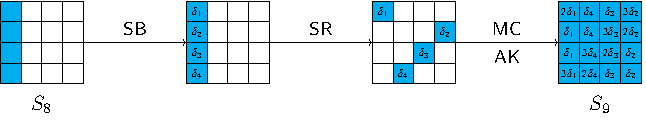
\includegraphics[width=0.9\textwidth]{fig/AES_Fault_Diagnol_Attack_Round_9.pdf}
    \caption{Visual illustration of fault propagation in the $9$th round of AES when the fault was injected in the diagonal $s_{00},s_{11},s_{22},s_{33}$ of the AES cipher state at the end of round $7$.
    $\delta_i$ ($i=1,2,3,4$) denote the differences between the four correct and faulty bytes in the first column of the cipher state after SubBytes in round $9$.}
\end{figure}
\[
\begin{pmatrix}
    \texttt{02} & \texttt{03} & \texttt{01} & \texttt{01} \\
    \texttt{01} & \texttt{02} & \texttt{03} & \texttt{01} \\
    \texttt{01} & \texttt{01} & \texttt{02} & \texttt{03} \\
    \texttt{03} & \texttt{01} & \texttt{01} & \texttt{02}
    \end{pmatrix}.
\]
\end{frame}

\begin{frame}{Notations}
    \begin{itemize}
        \item $S_9$: the cipher state at the end of round nine
        \item $c$: the correct ciphertext 
        \item $K_{10}$: the last round key $K_{10}$
   {\small \[
    S_9=
     \begin{pmatrix}
    a_{00} & a_{01} & a_{02} & a_{03}\\
    a_{10} & a_{11} & a_{12} & a_{13}\\
    a_{20} & a_{21} & a_{22} & a_{23}\\
    a_{30} & a_{31} & a_{32} & a_{33}
    \end{pmatrix},\ 
    c=
    \begin{pmatrix}
    c_{00} & c_{01} & c_{02} & c_{03}\\
    c_{10} & c_{11} & c_{12} & c_{13}\\
    c_{20} & c_{21} & c_{22} & c_{23}\\
    c_{30} & c_{31} & c_{32} & c_{33}
    \end{pmatrix},\
    K_{10}=
    \begin{pmatrix}
    k_{00} & k_{01} & k_{02} & k_{03}\\
    k_{10} & k_{11} & k_{12} & k_{13}\\
    k_{20} & k_{21} & k_{22} & k_{23}\\
    k_{30} & k_{31} & k_{32} & k_{33}
    \end{pmatrix}.
    \]}
    \item $c'$: faulty ciphertext
        \[
c'=
\begin{pmatrix}
    c'_{00} & c'_{01} & c'_{02} & c'_{03}\\
    c'_{10} & c'_{11} & c'_{12} & c'_{13}\\
    c'_{20} & c'_{21} & c'_{22} & c'_{23}\\
    c'_{30} & c'_{31} & c'_{32} & c'_{33}
    \end{pmatrix}.
\]
    \end{itemize}
\end{frame}

\begin{frame}{}
    \begin{itemize}
        \item Round $10$: SubBytes, ShiftRows, and AddRoundKey.
\[
c_{00}=\text{SB}_{\text{AES}}(a_{00})\oplus k_{00},\quad c_{13}=\text{SB}_{\text{AES}}(a_{10})\oplus k_{13},
\]
\[
c_{22}=\text{SB}_{\text{AES}}(a_{20})\oplus k_{22},\quad
c_{31}=\text{SB}_{\text{AES}}(a_{30})\oplus k_{31}.
\] 
\item Then
\begin{eqnarray*}
    a_{00} &=& \text{SB}_{\text{AES}}^{-1}(c_{00}\oplus k_{00})\\
    a_{10} &=& \text{SB}_{\text{AES}}^{-1}(c_{13}\oplus k_{13})\\
    a_{20} &=& \text{SB}_{\text{AES}}^{-1}(c_{22}\oplus k_{22})\\
    a_{30} &=& \text{SB}_{\text{AES}}^{-1}(c_{31}\oplus k_{31}).
\end{eqnarray*}
\item Similarly
\begin{eqnarray*}
    a'_{00} &=& \text{SB}_{\text{AES}}^{-1}(c'_{00}\oplus k_{00})\\
    a'_{10} &=& \text{SB}_{\text{AES}}^{-1}(c'_{13}\oplus k_{13})\\
    a'_{20} &=& \text{SB}_{\text{AES}}^{-1}(c'_{22}\oplus k_{22})\\
    a'_{30} &=& \text{SB}_{\text{AES}}^{-1}(c'_{31}\oplus k_{31}).
\end{eqnarray*}
    \end{itemize}
\end{frame}


\begin{frame}{}
    \begin{itemize}
\item Let $\delta=\delta_1$ and by observing the first column of $S_9$, we have
\begin{eqnarray*}
\texttt{2}\delta &=& a_{00}\oplus a'_{00}=\text{SB}_{\text{AES}}^{-1}(c_{00}\oplus k_{00})\oplus \text{SB}_{\text{AES}}^{-1}(c'_{00}\oplus k_{00})\\
\delta &=& a_{10}\oplus a'_{10}=\text{SB}_{\text{AES}}^{-1}(c_{13}\oplus k_{13})\oplus \text{SB}_{\text{AES}}^{-1}(c'_{13}\oplus k_{13})\\
\delta &=& a_{20}\oplus a'_{20}=\text{SB}_{\text{AES}}^{-1}(c_{22}\oplus k_{22})\oplus \text{SB}_{\text{AES}}^{-1}(c'_{22}\oplus k_{22})\\
\texttt{3}\delta &=& a_{30}\oplus a'_{30}=\text{SB}_{\text{AES}}^{-1}(c_{31}\oplus k_{31})\oplus \text{SB}_{\text{AES}}^{-1}(c'_{31}\oplus k_{31}).
\end{eqnarray*}
    \end{itemize}
\begin{figure}
    \centering
    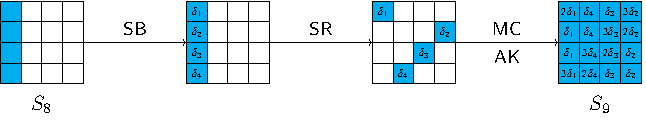
\includegraphics{fig/AES_Fault_Diagnol_Attack_Round_9.pdf}
\end{figure}
\end{frame}

\begin{frame}{Key recovery}
\begin{eqnarray*}
\texttt{2}\delta &=& a_{00}\oplus a'_{00}=\text{SB}_{\text{AES}}^{-1}(c_{00}\oplus k_{00})\oplus \text{SB}_{\text{AES}}^{-1}(c'_{00}\oplus k_{00})\\
\delta &=& a_{10}\oplus a'_{10}=\text{SB}_{\text{AES}}^{-1}(c_{13}\oplus k_{13})\oplus \text{SB}_{\text{AES}}^{-1}(c'_{13}\oplus k_{13})\\
\delta &=& a_{20}\oplus a'_{20}=\text{SB}_{\text{AES}}^{-1}(c_{22}\oplus k_{22})\oplus \text{SB}_{\text{AES}}^{-1}(c'_{22}\oplus k_{22})\\
\texttt{3}\delta &=& a_{30}\oplus a'_{30}=\text{SB}_{\text{AES}}^{-1}(c_{31}\oplus k_{31})\oplus \text{SB}_{\text{AES}}^{-1}(c'_{31}\oplus k_{31}).
\end{eqnarray*}
\begin{itemize}
    \item For each value of $\delta$, the possible values for $(k_{00},k_{13},k_{22},k_{31})$ are restricted
    \item $a_{00}=\text{SB}_{\text{AES}}^{-1}(c_{00}\oplus k_{00})$ can be considered as an AES Sbox input that corresponds to input difference $2\delta$ and output difference $c_{00}\oplus c'_{00}$
    \item $a_{10}=\text{SB}_{\text{AES}}^{-1}(c_{13}\oplus k_{13})$ is an AES Sbox input that gives output difference $c_{13}\oplus c'_{13}$ when the input difference is $\delta$
    \item On average\footnote{Saha, D., Mukhopadhyay, D., \& RoyChowdhury, D. (2009). A diagonal fault attack on the advanced encryption standard. Cryptology ePrint Archive.}, the key hypotheses for $(k_{00},k_{13},k_{22},k_{31})$ can be reduced to $2^8$
\end{itemize}
\end{frame}

\begin{frame}{Diagonal DFA}
    \begin{itemize}
        \item In this attack, we assume the attacker has the knowledge of
        \begin{itemize}
            \item the fault location: diagonal of cipher state at the end of round $7$
            \item fault model: random byte
            \item output of AES: correct and faulty ciphertext
        \end{itemize}
       \item Since the attack is on the diagonal of the cipher state, it is also called the \textit{diagonal DFA}.
    \end{itemize}
\end{frame}

\begin{frame}{Other diagonals}
\begin{figure}
    \centering
    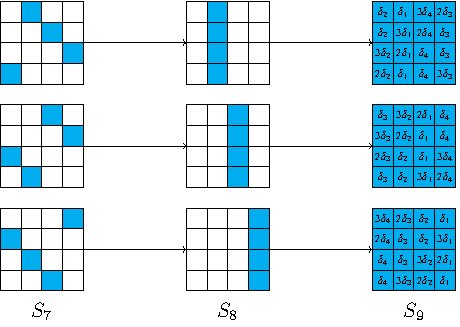
\includegraphics{fig/AES_DFA_all_diagonals.pdf}
    \caption{Fault propagation for random byte fault injected in the ``diagonals'' of the cipher state at the end of round $7$.
    $S_i$ denotes the cipher state at the end of the $i$th round}
\end{figure}
\end{frame}

\section{Other Fault Attacks}
\begin{frame}{\VideoName}
    \tableofcontents[currentsection]
\end{frame}

\begin{frame}{Ineffective Fault Analysis}
    \begin{itemize}
        \item Clavier, C. (2007, September). Secret external encodings do not prevent transient fault analysis. In International Workshop on Cryptographic Hardware and Embedded Systems (pp. 181-194). Springer, Berlin, Heidelberg. 
        \item Faults that do not change the intermediate values are exploited.
        \item Those faults are called \textit{ineffective faults}.
        \item Normally a particular fault model is assumed, e.g. a stuck-at-$0$ fault model.
    \end{itemize}
\end{frame}

\begin{frame}{Statistical Ineffective Fault Attack (SIFA)}
    \begin{itemize}
        \item Dobraunig, C., Eichlseder, M., Korak, T., Mangard, S., Mendel, F., \& Primas, R. (2018). SIFA: exploiting ineffective fault inductions on symmetric cryptography. IACR Transactions on Cryptographic Hardware and Embedded Systems, 547-572.
        \item A non-uniform fault model is assumed and the attack exploits ineffective faults.
        \item The dependency between the fault induction being ineffective and the data that is
processed is exploited.
        \item Different from SFA, SIFA does not require each fault to be successful, but the attack requires repeated plaintext, and knowledge of the correct ciphertext (or whether each ciphertext is correct or not).
        \item The fault injection is the same as for SFA
        \item In the original paper the authors provide a detailed theoretical analysis of the number of ciphertexts needed and extensive experimental results.
    \end{itemize}
\end{frame}

\begin{frame}{Persistent Fault Analysis (PFA)}
    \begin{itemize}
        \item Zhang, Fan, Xiaoxuan Lou, Xinjie Zhao, Shivam Bhasin, Wei He, Ruyi Ding, Samiya Qureshi, and Kui Ren. Persistent fault analysis on block ciphers. IACR Transactions on Cryptographic Hardware and Embedded Systems (2018): 150-172.
        \item Fault in the memory, Sbox lookup table
        \item Knowledge of ciphertext only
    \end{itemize}
\end{frame}

\begin{frame}{Algebraic Fault Analysis (AFA)}
    \begin{itemize}
        \item Courtois, N. T., Jackson, K., \& Ware, D. (2010). Fault-algebraic attacks on inner rounds of DES. In E-Smart'10 Proceedings: The Future of Digital Security Technologies. Strategies Telecom and Multimedia.
        \item Similar to DFA, exploits differences between correct and faulty ciphertext
        \item DFA -- manual analysis
        \item AFA -- expresses cryptographic algorithm in the form of algebraic equations and utilizes SAT solver\footnote{A SAT solver solves Boolean satisfiability problems.
It takes a Boolean logic formula and checks if there is a solution satisfying the formula.} to recover the key.
    \end{itemize}
\end{frame}

\begin{frame}{Collision Fault Analysis}
    \begin{itemize}
        \item Blömer, J., \& Seifert, J. P. (2003, January). Fault based cryptanalysis of the advanced encryption standard (AES). In International Conference on Financial Cryptography (pp. 162-181). Springer, Berlin, Heidelberg.
        \item Injects fault in the earlier rounds of a block cipher implementation.
        \item Then the attacker records the faulty ciphertext and finds plaintext that produces the same ciphertext, but without fault.
        \item Further analysis using those plaintexts can recover the round key.
        \item If the fault only changes one bit or one byte of the intermediate value, the attacker can try different plaintexts that only differ at one bit or one byte.
    \end{itemize}
\end{frame}

\begin{frame}{Fault Sensitivity Analysis}
    \begin{itemize}
        \item Li, Y., Sakiyama, K., Gomisawa, S., Fukunaga, T., Takahashi, J., \& Ohta, K. (2010, August). Fault sensitivity analysis. In International workshop on cryptographic hardware and embedded systems (pp. 320-334). Springer, Berlin, Heidelberg.
        \item Exploits the sensitivity of a device to faults
        \item The attack analyzes when a faulty output begins to exhibit some detectable characteristics and utilizes the information to recover the secret key.
        \item No knowledge of faulty ciphertext is required for the attack.
    \end{itemize}
\end{frame}
